\documentclass[12pt]{article}

\usepackage{hyperref}

% useful for formatting (align*, etc.) and for certain symbols (the QED box, etc.)
\usepackage{amsmath, amssymb, amsthm}

% for including graphics
\usepackage{graphicx}

% for conveniently specifying the spacing (\singlespacing, \doublespacing,
%    \onehalfspacing, etc.)
\usepackage{setspace}
\onehalfspacing

% this does some sort of symbol stuff
\usepackage{textcomp}

% A package for conveniently adjusting headers and such
\usepackage{fancyhdr}
\renewcommand{\headrulewidth}{0 pt}
\rhead{\textit{\thepage}}
\cfoot{}



% Set the margins
\usepackage[top=1.8cm, bottom=1.8cm, left=1.8cm, right=1.8cm]{geometry}

% Differently spaced itemize
\newenvironment{itemize*}%
  {\begin{itemize}%
  	\setlength{\parsep}{0pt}
    \setlength{\itemsep}{0pt}%
    \setlength{\parskip}{0pt}}%
  {\end{itemize}}
\newenvironment{enumerate*}%
  {\begin{enumerate}%
  	\setlength{\parsep}{0pt}
    \setlength{\itemsep}{0pt}%
    \setlength{\parskip}{0pt}}%
  {\end{enumerate}}


% set up a new command to insert a little bit of vertical space
% (use this BEFORE a line break)
\newcommand{\padding}{\vspace*{.5cm}}

% set up an environment to format each hw problem in
\newenvironment{problem}[1]{\noindent\textbf{#1.}}{\vspace*{.5cm}}

\newenvironment{proof*}{\par\noindent{\bf Proof}\quad}
               {\quad\vrule height 8pt depth 0pt width 8pt\medskip\par}



\begin{document}

\section{User Documentation}
\subsection{Features Overview}
 VirPong provides a safe and fun pong game that combines the use of connections and communication between Wii Remotes, smart phones, and a local University of Puget Sound Server. This allows you to play pong against another human player using your phone and a Wii Remote as a controller.

\subsection{Setting Up}
Setting up VirPong game environment and account is simple and quick. It allows for the convenient set up of everything entirely from your phone through the use of our website.
\begin{itemize}
\item The product can be downloaded by directing your Android internet browser to “WEBSITE” and clicking on the Android APK download. An automatic prompt asking if you want to install the APK should pop up. Follow your phones instructions to complete installation of the application.
\item Follow the instructions on the website to quickly and easily set up your own VirPong user account, information, and password. If you do not want to do this, you also have the choice of not logging in and using a guest account.
\item Once your user account has been set up launch the application.
\end{itemize}
\subsection{Functions of the Main Menu}
\begin{figure}
\begin{center}
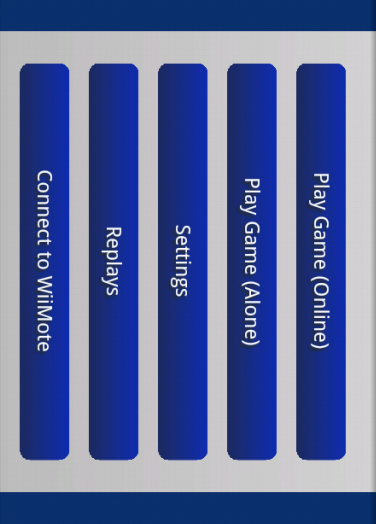
\includegraphics[scale=.7]{homeScreen.png}
\caption{\label{homeScreen}Home Screen Menu}
\end{center}
\end{figure}

\subsubsection{User Settings}
\begin{figure}
\begin{center}
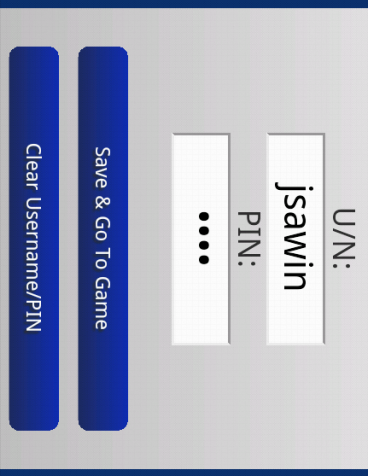
\includegraphics[scale=.7]{userNamePinSave.png}
\caption{\label{User Setting Interface}User Settings Menu}
\end{center}
\end{figure}

The first thing a user will probably want to do upon opening the application for the first time is opening the settings page. This will bring up a page that allows the user to put in their username and pin number that will save so they can stay logged in through multiple uses.
\subsubsection{Select Input Method}
\begin{figure}
\begin{center}
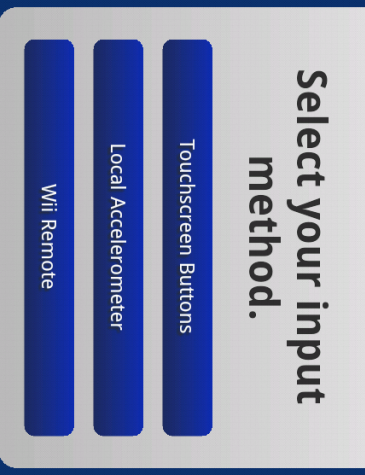
\includegraphics[scale=.7]{selectInputMethod-Android.png}
\caption{\label{Input Selection Interface}Input Selection Menu}
\end{center}
\end{figure}

After saving any settings, the user will want to select the input method and follow the correct steps to set up the input device.
\begin{itemize}
\item Wii Remote – choose this under input options and run the plugin in order to use a Wii Remote as your controller. The plugin should pop up and allow you to connect to the Wii Remote. Once connection has been verified you are ready to play a game.
\item Phone Accelerometer – this option will allow you to use the phones accelerometer rather than the Wii Remote. This allows you to play if you don’t have a Wii Remote.
\item Button Presses – choosing this input method will allow you to play the game by using button presses on the screen to move your paddle.
\end{itemize}
\subsubsection{Play Game}
Upon selecting the Play Game on Internet option, the application will bring you to a page containing different game rooms. 
\begin{figure}
\begin{center}
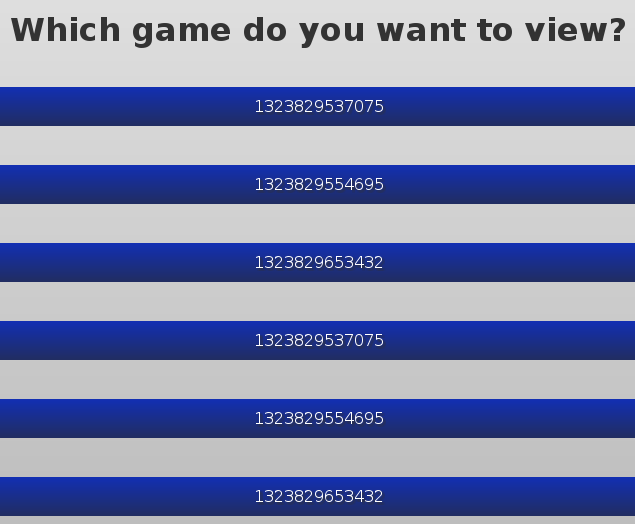
\includegraphics[scale=.7]{gameSelect.png}
\caption{\label{gameSelection}List of Joinable Games Menu}
\end{center}
\end{figure}

\begin{itemize}
\item Choosing a game with one person already in it will allow you to join the game and start playing versus them.
\item You can choose to create a new game, where you will have to wait until another player joins to start.
\item Or you can join a game that already has two players and watch them play as an observer.
\end{itemize}
You can also choose to play offline against a simple bot program in order to test your skills when an opponent is no longer available.
\begin{figure}
\begin{center}
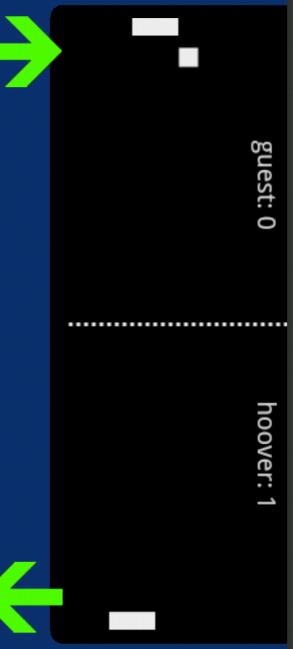
\includegraphics[scale=.7]{touchOnServer.png}
\caption{\label{PlayingGame}Game in Action}
\end{center}
\end{figure}

\subsubsection{Replay Game}
After you have played a game or even if you haven’t and just want to watch a replay of a game, select the function to watch a replay. This will bring up a selection of previously played games to watch from.
\subsection{Rules of Pong}
Now for the fun, playing pong is extremely simple and fun. The rules are straight forward and any new player can pick them up easily. Here are the basics:
\subsubsection {Major Components}
There are 3 major components to any pong game. These are the ball, the paddles, and score area. 
\begin{itemize}
\item Ball – flies around the screen following basic game mechanics and doing basic collision detection. If this makes it into your score area, you lose a point.
\item Score area – this is everything between your paddle and the end of the screen. 
\item Paddle – this is the only thing the user controls. The game will tell you which of the two is yours and use of your selected input method will cause it to move up and down on the screen. 
\end{itemize}
\subsubsection{How to Play}
The basic concept of a pong game is to hit the ball with your paddle more than your opponent does. Try to send the ball flying into your opponents score area while still defending your score area from balls your opponent sends flying at you. The first to 10 points wins.



\end{document}